% =====================================================================
%  Rapport technique - Ingenierie DevSecOps
%  Compilation : pdfLaTeX (Overleaf)
%  Images : cherchees dans ../captures/ puis dans le dossier courant,
%           afin de fonctionner aussi bien depuis le depot que depuis
%           un dossier Overleaf a plat.
% =====================================================================
\documentclass[11pt,a4paper]{article}

\usepackage[utf8]{inputenc}
\usepackage[T1]{fontenc}
\usepackage[french]{babel}
\usepackage{lmodern}
\usepackage[a4paper,margin=2.4cm]{geometry}

\usepackage{amssymb}
\usepackage{graphicx}
\graphicspath{{../captures/}{./}{captures/}}

\usepackage{xcolor}
\usepackage{booktabs}
\usepackage{tabularx}
\usepackage{array}
\usepackage{longtable}
\usepackage{enumitem}
\usepackage{caption}
\usepackage{fancyhdr}
\usepackage{listings}
\usepackage{tikz}
\usetikzlibrary{positioning,arrows.meta,shapes.geometric,fit,backgrounds,calc}

% ---------------------------------------------------------------------
%  Palette : definie avant hyperref, qui s'en sert pour les liens.
% ---------------------------------------------------------------------
\definecolor{bleuFonce}{HTML}{1F4E79}
\definecolor{bleuClair}{HTML}{DEEAF6}
\definecolor{grisFonce}{HTML}{404040}
\definecolor{grisClair}{HTML}{F2F2F2}
\definecolor{vertOk}{HTML}{2E7D32}
\definecolor{rougeAlerte}{HTML}{B3261E}
\definecolor{orangeAcc}{HTML}{B26500}

\usepackage{hyperref}
\hypersetup{
  colorlinks=true,
  linkcolor=bleuFonce,
  urlcolor=bleuFonce,
  citecolor=bleuFonce,
  pdftitle={Rapport technique - Ingenierie DevSecOps},
  pdfauthor={Aissatou Lo}
}

% ---------------------------------------------------------------------
%  Mise en page
% ---------------------------------------------------------------------
\pagestyle{fancy}
\fancyhf{}
\fancyhead[L]{\small\color{grisFonce}Ingénierie DevSecOps — Plateforme E-Commerce}
\fancyhead[R]{\small\color{grisFonce}\thepage}
\renewcommand{\headrulewidth}{0.4pt}

\captionsetup{font=small,labelfont=bf}
\setlist{itemsep=2pt,topsep=4pt}

\newcolumntype{L}[1]{>{\raggedright\arraybackslash}p{#1}}

% Fragment de code en ligne. babel-french rend ':' ';' '!' '?' actifs pour
% inserer l'espace fine que veut la typographie francaise : correct en prose,
% faux dans du code, ou cela produirait « @sha256 :... ». On desactive donc
% ces raccourcis a l'interieur des fragments techniques uniquement.
\newcommand{\code}[1]{{\shorthandoff{:;!?}\texttt{#1}}}

% Pastille de gain. Les quatre categories sont exactement celles du sujet :
% vitesse, fiabilite, cout, securite.
\newcommand{\pastille}[2]{%
  \colorbox{#1}{\color{white}\scriptsize\bfseries\strut #2}}
\newcommand{\gVitesse}{\pastille{bleuFonce}{VITESSE}}
\newcommand{\gFiabilite}{\pastille{vertOk}{FIABILITÉ}}
\newcommand{\gSecurite}{\pastille{rougeAlerte}{SÉCURITÉ}}
\newcommand{\gCout}{\pastille{orangeAcc}{COÛT}}

% Marqueur d'etape bloquante
\newcommand{\bloque}{\textcolor{rougeAlerte}{$\checkmark$}}
\newcommand{\nonbloque}{\textcolor{grisFonce}{--}}

% Encadre pour les points saillants
\newcommand{\encadre}[2]{%
  \begin{center}
  \fcolorbox{bleuFonce}{bleuClair}{%
    \begin{minipage}{0.94\linewidth}
      \vspace{2pt}
      \textbf{#1}\par\vspace{3pt}#2
      \vspace{2pt}
    \end{minipage}}
  \end{center}}

% ---------------------------------------------------------------------
%  Style des extraits de code
% ---------------------------------------------------------------------
\lstdefinestyle{conf}{
  basicstyle=\ttfamily\footnotesize,
  keywordstyle=\color{bleuFonce}\bfseries,
  commentstyle=\color{grisFonce}\itshape,
  stringstyle=\color{vertOk},
  backgroundcolor=\color{grisClair},
  frame=single,
  rulecolor=\color{grisFonce!40},
  breaklines=true,
  showstringspaces=false,
  columns=flexible,
  xleftmargin=8pt,
  framexleftmargin=8pt,
  aboveskip=10pt,
  belowskip=10pt
}
\lstset{style=conf}

% ---------------------------------------------------------------------
%  Styles TikZ communs aux deux diagrammes
% ---------------------------------------------------------------------
\tikzset{
  bloc/.style={
    rectangle, rounded corners=2pt, draw=bleuFonce, fill=bleuClair,
    text width=26mm, align=center, minimum height=11mm,
    font=\footnotesize, inner sep=3pt},
  blocGris/.style={bloc, draw=grisFonce, fill=grisClair},
  blocVert/.style={bloc, draw=vertOk, fill=vertOk!10},
  blocRouge/.style={bloc, draw=rougeAlerte, fill=rougeAlerte!8},
  decision/.style={
    diamond, aspect=2.2, draw=orangeAcc, fill=orangeAcc!12,
    text width=17mm, align=center, font=\scriptsize, inner sep=1pt},
  fleche/.style={-{Stealth[length=2mm]}, draw=grisFonce, thick},
  flechePointillee/.style={fleche, dashed},
  etiquette/.style={font=\scriptsize\itshape, color=grisFonce}
}

% =====================================================================
\begin{document}

% ---------------------------------------------------------------------
%  Page de titre
% ---------------------------------------------------------------------
\begin{titlepage}
\centering
\vspace*{2cm}

{\color{grisFonce}\large EXAMEN / PROJET DEVSECOPS\par}
\vspace{4mm}
{\color{bleuFonce}\rule{\linewidth}{1.2pt}}
\vspace{8mm}

{\Huge\bfseries Ingénierie DevSecOps\par}
\vspace{5mm}
{\LARGE Déploiement d'une plateforme\\E-Commerce moderne\par}

\vspace{6mm}
{\color{bleuFonce}\rule{\linewidth}{1.2pt}}

\vspace{14mm}
{\large\itshape « Le DevOps ne se résume pas à l'automatisation de la même
façon que l'astronomie ne se résume pas aux télescopes. »\par}

\vspace{18mm}
\begin{tabular}{rl}
  \textbf{Auteur} & Aissatou Lo\\[3pt]
  \textbf{Module} & DevOps / DevSecOps\\[3pt]
  \textbf{Application} & \url{https://examdevsecops.onrender.com}\\[3pt]
  \textbf{Dépôt} & \url{https://github.com/aissatoulo427/examdevsecops}\\[3pt]
  \textbf{Registre} & \texttt{ghcr.io/aissatoulo427/examdevsecops}\\
\end{tabular}

\vfill
{\color{grisFonce}\today}
\end{titlepage}

\tableofcontents
\newpage

% =====================================================================
\section{Contexte et objectifs}
% =====================================================================

Le sujet demande une plateforme e-commerce moderne consommant la Fake Store
API. Son cœur n'est pourtant pas l'application, mais \textbf{la chaîne de
valeur} qui la porte du code source jusqu'à l'utilisateur, et le retour
d'information qui remonte dans l'autre sens.

L'application est donc restée volontairement simple — authentification,
catalogue, panier — pour que l'effort porte là où il est évalué : le
pipeline, la sécurité et l'observabilité. Une application riche accompagnée
d'une chaîne pauvre répondrait à côté de la question posée.

Quatre objectifs ont guidé chaque décision et servent de grille de lecture à
l'ensemble du rapport. Chaque choix technique présenté par la suite est
rattaché à au moins l'un d'eux.

\begin{table}[htbp]
\centering
\begin{tabularx}{\linewidth}{@{}l X@{}}
\toprule
\textbf{Objectif} & \textbf{Traduction concrète} \\
\midrule
Vitesse & Une modification fusionnée est en ligne sans intervention manuelle ; les défauts sont signalés en secondes, pas en revue de code. \\
Fiabilité & Un pipeline vert signifie que le service répond réellement ; il n'échoue jamais pour une cause extérieure au dépôt. \\
Sécurité & Aucun secret dans le dépôt ni dans l'image ; rien n'est publié sans avoir été scanné au préalable. \\
Reproductibilité & Un tiers reconstruit et exécute l'ensemble — application, pipeline, observabilité — à partir du dépôt seul. \\
\bottomrule
\end{tabularx}
\caption{Les quatre objectifs directeurs}
\end{table}

Le dernier objectif est celui qui a le plus modelé l'architecture. Il impose
que rien de ce qui fait fonctionner la chaîne ne réside en dehors du dépôt :
ni configuration cachée, ni service à installer manuellement, ni étape
connue du seul auteur.

% =====================================================================
\subsection*{Correspondance avec les attendus du sujet}

\begin{table}[htbp]
\centering
\small
\begin{tabular}{@{}c l l@{}}
\toprule
\textbf{N\textsuperscript{o}} & \textbf{Livrable attendu} & \textbf{Où il est traité} \\
\midrule
1 & Rapport technique               & Ce document \\
2 & Diagrammes architecture et chaîne de valeur & Figures des sections 2 et 3 \\
3 & Dépôt Git : code et configurations & Lien en page de titre \\
4 & Pipeline CI/CD fonctionnel      & Section 3 · \code{.github/workflows/ci.yml} \\
5 & Tests automatisés               & Section 5 · \code{src/**/*.test.ts(x)} \\
6 & Configurations de sécurité      & Section 4 · \code{Dockerfile}, \code{nginx.conf}, \\
  &                                 & \code{.gitleaks.toml}, \code{sonar-project.properties} \\
7 & Stratégie d'observabilité       & Section 6 · \code{observability/} \\
8 & Conclusion : limites et améliorations & Section 7 \\
\bottomrule
\end{tabular}
\caption{Les huit livrables du sujet et leur emplacement}
\label{tab:livrables}
\end{table}

Le schéma d'architecture de la section suivante contient les sept éléments
exigés au minimum par le sujet : utilisateur, frontend conteneurisé, API
Fake Store, pipeline CI/CD, registre d'images, outils de sécurité et système
d'observabilité.

% =====================================================================
\section{Architecture retenue}
% =====================================================================

\subsection{Vue d'ensemble}

Une application React~19 construite par Vite, servie en fichiers statiques
par nginx dans un conteneur durci, déployée sur une plateforme d'hébergement
conteneurisé. Le navigateur appelle la Fake Store API \textbf{directement},
sans backend intermédiaire. GitHub~Actions contrôle, teste, scanne,
construit et publie l'image sur GHCR, puis déclenche le déploiement. Une
pile Prometheus / Grafana / blackbox-exporter, exécutable localement, sonde
l'URL publique depuis l'extérieur.

\begin{figure}[htbp]
\centering
\begin{tikzpicture}

  % --- Rang median : le chemin de l'utilisateur
  \node[bloc]      (U) at ( 0,   0)   {Utilisateur\\(navigateur)};
  \node[bloc]      (R) at ( 5,   0)   {Frontend conteneurisé\\nginx + build React};
  \node[bloc]      (F) at (10,   0)   {Fake Store API\\\texttt{fakestoreapi.com}};

  % --- Rang inferieur : la chaine de livraison
  \node[bloc]      (G) at ( 0,  -3.5) {Pipeline CI/CD\\GitHub Actions};
  \node[bloc]      (H) at ( 5,  -3.5) {Registre d'images\\GHCR};
  \node[blocVert]  (O) at (10,  -3.5) {Observabilité\\Prometheus · Grafana\\blackbox};
  \node[blocRouge] (S) at ( 0,  -6.6) {Outils de sécurité\\Gitleaks · Trivy\\SonarQube};

  % --- Trafic utilisateur
  \draw[fleche] (U) -- node[etiquette, above] {HTTPS} (R);
  \draw[fleche] (U.north) -- (0,1.8)
        -- node[etiquette, above] {appels API directs (HTTPS)} (10,1.8) -- (F.north);

  % --- Chaine de livraison
  \draw[fleche] (G) -- node[etiquette, left]  {exécute} (S);
  \draw[fleche] (G) -- node[etiquette, above] {publie l'image} (H);
  \draw[fleche] (H.north) -- node[etiquette, right] {image} (R.south);
  \draw[fleche] (G.north) -- node[etiquette, left, pos=0.6] {deploy hook} (R.south west);

  % --- Retour d'information
  \draw[fleche] (O.north) -- node[etiquette, right] {sonde externe} (R.south east);

\end{tikzpicture}
\caption{Architecture cible. Les sept éléments demandés par le sujet
apparaissent : utilisateur, frontend conteneurisé, API Fake Store, pipeline
CI/CD, registre d'images, outils de sécurité et système d'observabilité.}
\end{figure}

\subsection{Le trajet d'une modification}

Une modification part d'une branche et d'une pull request. La poussée
déclenche le workflow, qui exécute d'abord le contrôle de la source : lint,
vérification des types, tests avec seuil de couverture, détection de
secrets, scan des dépendances, puis Quality Gate. Tant que la pull request
est ouverte, rien n'est publié et rien n'est déployé.

Si tout passe, l'image Docker est construite \emph{localement}, soumise à
Trivy, et poussée sur GHCR seulement ensuite — et seulement depuis la
branche principale. Après fusion, le déploiement est déclenché, puis le
pipeline attend et vérifie que l'URL publique répond avant de se déclarer
vert.

\subsection{Décisions structurantes}

\paragraph{Aucun backend.} Le navigateur appelle la Fake Store API
directement. C'est fidèle au sujet et cela supprime une surface d'attaque
entière : pas de service intermédiaire à construire, scanner, déployer,
observer ni maintenir. La contrepartie est que le jeton
d'authentification vit côté client, limite traitée en
section~\ref{sec:securite} et reprise en conclusion.

\paragraph{Frontend conteneurisé, et non site statique.} Un hébergement de
site statique aurait été plus simple et plus rapide à mettre en ligne. Il a
été écarté parce que le sujet demande explicitement un frontend
\emph{conteneurisé} dans le schéma d'architecture : ce choix aurait fait
disparaître le \texttt{Dockerfile}, le durcissement de l'image et son scan —
c'est-à-dire une part substantielle de ce qui est évalué. Le coût assumé est
un déploiement plus long, puisque l'image doit être reconstruite.

\paragraph{Analyse de qualité confiée à un service géré.} SonarQube Cloud
est gratuit pour les dépôts publics. Une instance auto-hébergée aurait
imposé de gérer un serveur, sa disponibilité, ses mises à jour et des
secrets d'authentification supplémentaires. Le service géré ramène
l'authentification à un seul jeton et, surtout, \textbf{supprime toute
dépendance à une infrastructure particulière} : c'est ce que le sujet entend
par reproductible.

\encadre{Conséquence directe sur la reproductibilité}{%
La chaîne complète se rejoue à partir du dépôt seul. Aucun serveur à
provisionner, aucune installation préalable, aucune étape connue du seul
auteur. Un correcteur peut cloner, construire l'image, lancer la pile
d'observabilité et lire le pipeline sans rien demander à personne.}

% =====================================================================
\section{La chaîne CI/CD étape par étape}
% =====================================================================

Un seul workflow, \texttt{.github/workflows/ci.yml}, déclenché sur pull
request et sur poussée vers la branche principale. Trois tâches enchaînées :
qualité, image, déploiement.

\begin{figure}[htbp]
\centering
\begin{tikzpicture}[node distance=6mm]

  % --- Colonne 1 : controle de la source
  \node[bloc] (c1) {Commit / PR};
  \node[bloc, below=of c1] (c2) {Lint};
  \node[bloc, below=of c2] (c3) {Vérification\\des types};
  \node[bloc, below=of c3] (c4) {Tests\\+ couverture};
  \node[blocRouge, below=of c4] (c5) {Gitleaks\\(secrets)};
  \node[blocRouge, below=of c5] (c6) {Trivy \texttt{fs}\\(dépendances)};
  \node[bloc, below=of c6] (c7) {SonarQube\\Quality Gate};

  \foreach \a/\b in {c1/c2, c2/c3, c3/c4, c4/c5, c5/c6, c6/c7}
    \draw[fleche] (\a) -- (\b);

  % --- Colonne 2 : image et deploiement
  \node[bloc, right=32mm of c2] (i1) {Build image\\(local)};
  \node[blocRouge, below=of i1] (i2) {Trivy \texttt{image}\\(paquets système)};
  \node[bloc, below=of i2] (i3) {Publication\\GHCR};
  \node[decision, below=8mm of i3] (d1) {branche\\principale ?};
  \node[bloc, below=8mm of d1] (p1) {Déploiement\\(deploy hook)};
  \node[blocVert, below=of p1] (p2) {Vérification\\\texttt{/healthz}};

  \draw[fleche] (i1) -- (i2);
  \draw[fleche] (i2) -- (i3);
  \draw[fleche] (i3) -- (d1);
  \draw[fleche] (d1) -- node[etiquette, right] {oui} (p1);
  \draw[fleche] (p1) -- (p2);
  \node[blocGris, right=10mm of d1] (stop) {Arrêt};
  \draw[fleche] (d1) -- node[etiquette, above] {non} (stop);

  % --- Liaison entre les deux colonnes
  \draw[fleche] (c7.east) -- ++(8mm,0) |- (i1.west);

  % --- Cadres de regroupement
  \begin{scope}[on background layer]
    \node[draw=grisFonce!50, dashed, rounded corners, fit=(c1)(c7),
          inner sep=4mm, label={[etiquette]above:Contrôle de la source}] {};
    \node[draw=grisFonce!50, dashed, rounded corners, fit=(i1)(i3),
          inner sep=4mm, label={[etiquette]above:Image}] {};
    \node[draw=grisFonce!50, dashed, rounded corners, fit=(p1)(p2),
          inner sep=4mm, label={[etiquette]below:Mise en ligne}] {};
  \end{scope}

\end{tikzpicture}
\caption{Chaîne de valeur. Les étapes en rouge sont les barrières de
sécurité ; l'étape en vert est celle qui transforme « le pipeline est vert »
en « l'utilisateur est servi ».}
\end{figure}

\subsection{Les onze étapes et leur gain}

\begin{table}[htbp]
\centering
\small
\begin{tabular}{@{}l l c l@{}}
\toprule
\textbf{Étape} & \textbf{Outil} & \textbf{Bloquante} & \textbf{Gain visé} \\
\midrule
Lint                 & oxlint              & \bloque    & \gVitesse   \\
Vérification des types & \texttt{tsc}      & \bloque    & \gFiabilite \\
Tests et couverture  & Vitest + MSW        & \bloque    & \gFiabilite \\
Détection de secrets & Gitleaks            & \bloque    & \gSecurite  \\
Scan des dépendances & Trivy \texttt{fs}   & \bloque    & \gSecurite  \\
Qualité et SAST      & SonarQube           & \bloque    & \gFiabilite \\
Construction image   & Buildx + cache      & \bloque    & \gCout      \\
Scan de l'image      & Trivy \texttt{image} & \bloque   & \gSecurite  \\
Publication          & GHCR                & \nonbloque & \gSecurite  \\
Déploiement          & Deploy hook         & \bloque    & \gVitesse   \\
Vérification en ligne & \texttt{curl /healthz} & \bloque & \gFiabilite \\
\bottomrule
\end{tabular}
\caption{Les onze étapes du pipeline. Les catégories de gain sont celles du
sujet : vitesse, fiabilité, coût, sécurité.}
\label{tab:etapes}
\end{table}

\textbf{Pourquoi cet ordre.} Les étapes sont classées par coût croissant :
une erreur de syntaxe ne doit pas coûter un build d'image pour être
découverte. Le lint et les types répondent en secondes ; les tests demandent
l'installation des dépendances mais restent hors réseau ; le build d'image
n'intervient qu'une fois la source entièrement validée.

\textbf{Pourquoi ces barrières.} La détection de secrets précède tout ce qui
publie : un secret publié est compromis, c'est le seul défaut qu'un
correctif ultérieur ne rattrape pas. Les deux scans Trivy sont
complémentaires et non redondants — le premier voit les dépendances du
projet, le second les paquets système de l'image de base.

\textbf{Ce qui n'est pas bloquant.} Seule la publication ne l'est pas : elle
n'est pas un contrôle mais une conséquence. Les deux dernières étapes ne
s'exécutent que depuis la branche principale — une pull request est
contrôlée de bout en bout, mais ne publie ni ne déploie rien.

\subsection{Trois points d'implémentation}

\paragraph{L'image est scannée avant d'être publiée, jamais l'inverse.}
Elle est d'abord construite localement, puis soumise à Trivy, et poussée
seulement ensuite. Publier puis scanner laisserait une image vulnérable
téléchargeable pendant l'intervalle, aussi bref soit-il — et un registre
public n'oublie pas ce qui y a été poussé.

\paragraph{Gitleaks inspecte l'historique complet.} Cela impose
\code{fetch-depth: 0} au checkout. Se limiter au diff de la pull request
laisserait passer un secret introduit puis supprimé dans la même branche,
alors qu'il reste lisible dans l'historique, donc compromis.

\paragraph{Le déploiement n'est acquis qu'après vérification.} Un hook
accepté est une promesse, pas une mise en ligne. Le pipeline attend la
reconstruction puis sonde \texttt{/healthz} jusqu'à obtenir un
\texttt{200}. Cette étape n'a pas été ajoutée par principe : elle vient d'un
incident réel où nginx refusait de démarrer alors que le pipeline restait
vert.

% =====================================================================
\section{Stratégie de sécurité}
\label{sec:securite}
% =====================================================================

La sécurité n'est pas une étape du pipeline, c'est une propriété qui doit
tenir à quatre niveaux. Chacun a ses défaillances propres, qu'aucun des
trois autres ne rattrape.

\subsection{Niveau 1 — le code}

SonarQube Cloud applique une Quality Gate bloquante : bugs, \textit{code
smells}, vulnérabilités, duplication. \texttt{oxlint} et la vérification des
types complètent en amont.

Le point important n'est pas l'outil mais le caractère \textbf{bloquant} de
la porte. Un rapport de qualité consultatif est lu les premières semaines
puis ignoré ; une porte qui refuse la fusion est la seule forme de règle qui
tienne dans la durée.

\subsection{Niveau 2 — les secrets}

\begin{table}[htbp]
\centering
\small
\begin{tabular}{@{}l l l@{}}
\toprule
\textbf{Secret} & \textbf{Portée} & \textbf{Usage} \\
\midrule
\texttt{SONAR\_TOKEN}            & dépôt                      & Analyse SonarQube \\
\texttt{RENDER\_DEPLOY\_HOOK\_URL} & environnement \texttt{production} & Déclenchement du déploiement \\
\texttt{GITHUB\_TOKEN}           & fourni par tâche           & Publication sur GHCR \\
\bottomrule
\end{tabular}
\caption{Inventaire complet des secrets : trois, aucun dans le dépôt}
\end{table}

\textbf{Gitleaks étend le jeu de règles par défaut} au lieu de le remplacer :
une configuration écrite de zéro perdrait silencieusement les centaines de
règles maintenues en amont, et une régression silencieuse dans un outil de
sécurité est pire que son absence. Les deux exclusions déclarées le sont
\textbf{par valeur exacte et non par chemin} — exclure un fichier créerait
une zone aveugle permanente, alors qu'un vrai secret déposé dans ces mêmes
fichiers reste détecté.

\textbf{Le secret de déploiement est porté par un environnement GitHub}, non
par le dépôt. La différence est de nature : une pull request, même ouverte
depuis un fork, ne peut ni le lire ni déclencher de déploiement. Sans cela,
un contributeur extérieur exfiltrerait l'URL du hook par une simple
modification du workflow.

\begin{figure}[htbp]
\centering
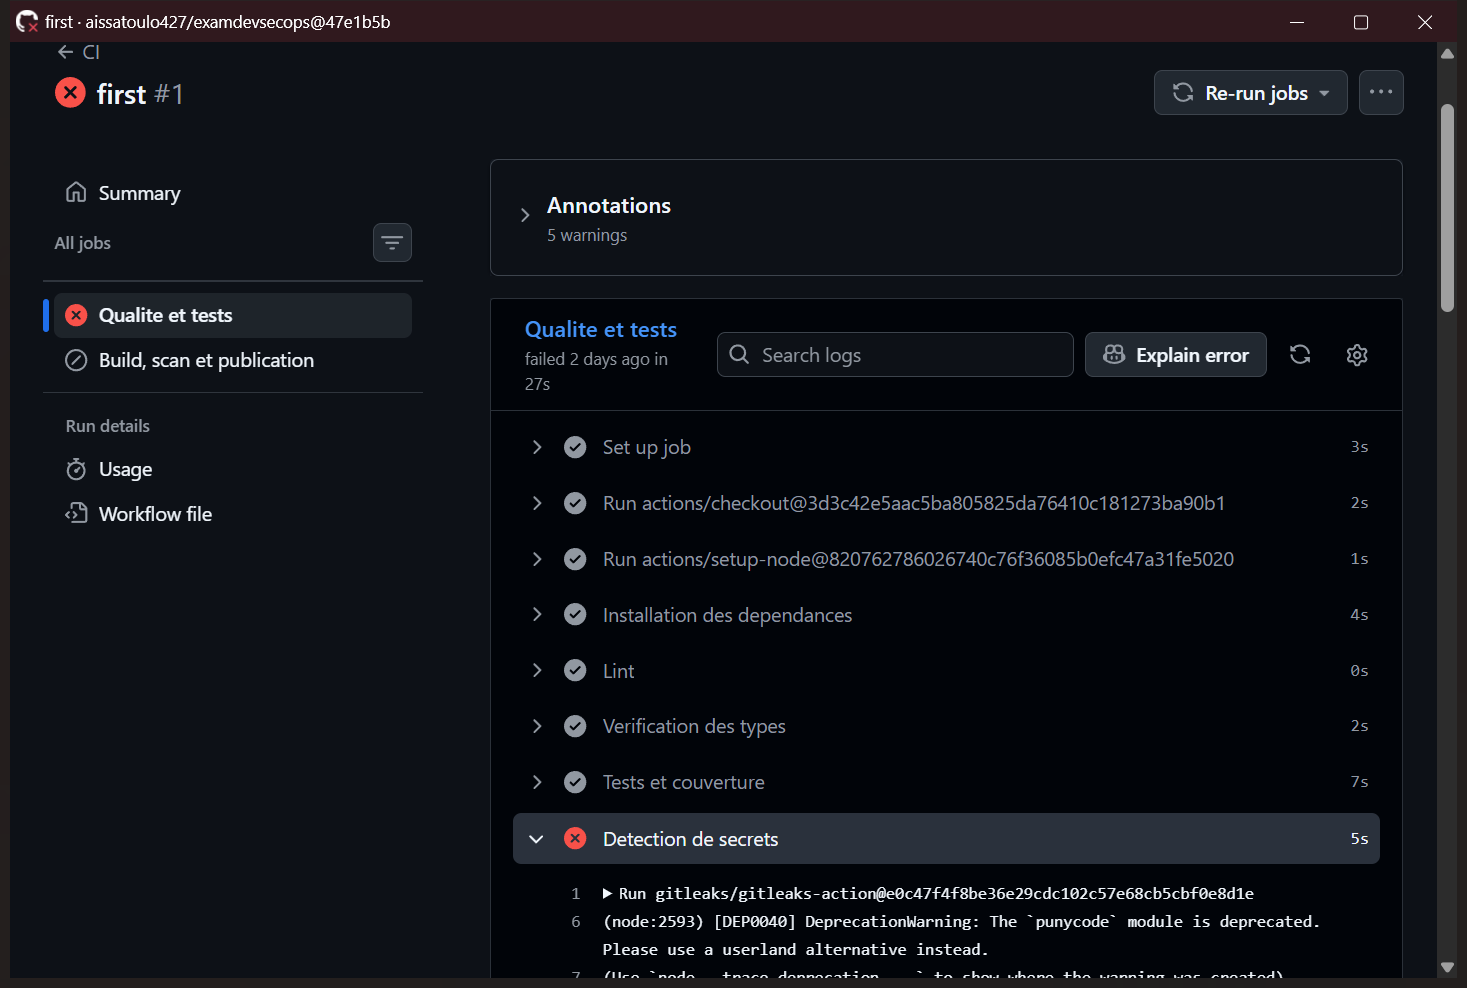
\includegraphics[width=\linewidth]{gitleaks-blocage.png}
\caption{Détection de secrets bloquant le pipeline. Toutes les étapes
antérieures sont vertes ; l'échec interrompt la tâche et la publication de
l'image n'est jamais atteinte.}
\end{figure}

\subsection{Niveau 3 — la chaîne d'approvisionnement}

Le niveau le plus souvent négligé, et celui où une compromission est la plus
difficile à détecter : le code du dépôt reste inchangé.

\begin{table}[htbp]
\centering
\small
\begin{tabular}{@{}l l@{}}
\toprule
\textbf{Mesure} & \textbf{Ce qu'elle empêche} \\
\midrule
Images de base épinglées par digest & Un tag redirigé vers un autre contenu \\
Actions épinglées par SHA de commit & Le même détournement, côté CI \\
\texttt{npm ci} plutôt que \texttt{npm install} & Une version non verrouillée \\
Trivy sur la source \emph{et} sur l'image & Deux surfaces distinctes, aucune seule suffisante \\
Permissions minimales par tâche & Un jeton large exploité par une dépendance \\
Concurrence limitée & Une exécution ancienne déployant après une récente \\
\bottomrule
\end{tabular}
\caption{Six mesures contre la compromission de la chaîne d'approvisionnement}
\end{table}

Une action tierce s'exécute avec l'accès au dépôt et aux secrets de la
tâche : c'est du code de confiance, il doit être figé comme tel.

\encadre{Un compromis assumé}{%
L'image applique les correctifs système publiés depuis la construction de
l'image de base — sans quoi le scan bloque la publication pour des
vulnérabilités déjà corrigées en amont. Cela \textbf{affaiblit la
reproductibilité bit à bit}, la version des paquets dépendant de la date de
build. Entre une image reproductible et vulnérable et une image corrigée
dont l'empreinte varie, le second terme a été retenu.}

\subsection{Niveau 4 — l'exécution}

\begin{itemize}
  \item Exécution \textbf{non-root}, sur le port 8080 — un processus non
        privilégié ne peut se lier sous 1024.
  \item Système de fichiers racine en \textbf{lecture seule},
        \texttt{no-new-privileges}, abandon de toutes les capacités.
  \item \texttt{.dockerignore} empêchant tout fichier d'environnement
        d'entrer dans le contexte de build.
  \item Cinq en-têtes de sécurité servis par nginx.
\end{itemize}

Le plus significatif est la \textit{Content-Security-Policy} :

\begin{lstlisting}
connect-src 'self' https://fakestoreapi.com
\end{lstlisting}

C'est la traduction en politique navigateur d'un fait d'architecture :
l'application n'a qu'une seule sortie réseau légitime. Un script injecté ne
pourrait exfiltrer de données vers aucune autre destination.

Enfin, le jeton \textbf{ne va jamais dans \texttt{localStorage}} — celui-ci
survivrait à la fermeture de l'onglet et resterait lisible par tout script
sur l'origine. Un test dédié vérifie cette propriété, pour qu'une régression
soit signalée par le pipeline plutôt que découverte en production.

% =====================================================================
\section{Stratégie de test}
% =====================================================================

\begin{table}[htbp]
\centering
\begin{tabularx}{\linewidth}{@{}l l X@{}}
\toprule
\textbf{Niveau} & \textbf{Outil} & \textbf{Ce qui est couvert} \\
\midrule
Unitaire & Vitest & Réducteur du panier : ajout, retrait, quantités, total, cas limites \\
Unitaire & Vitest & Service d'authentification : succès, échec, absence du jeton dans \texttt{localStorage} \\
Composant & Testing Library & Catalogue, formulaire de connexion, page panier, garde de route \\
Réseau & MSW & Interception de tous les appels à la Fake Store API \\
\bottomrule
\end{tabularx}
\caption{41 tests répartis sur 7 fichiers, exécutés à chaque poussée}
\end{table}

\subsection{Un seuil de couverture ciblé, et non global}

Le seuil bloquant est fixé à \textbf{80\,\% de lignes et de branches sur la
logique du panier et sur l'authentification} uniquement, sans seuil global.

C'est un choix, pas un renoncement. Un seuil global élevé pousse
mécaniquement à écrire des tests de rendu sans valeur — monter un composant,
vérifier qu'il ne plante pas — pour atteindre un chiffre. Le résultat est
une couverture flatteuse et une suite qui ne détecte rien. En ciblant le
calcul d'un total et le traitement d'un jeton, le seuil protège exactement
ce dont la régression coûte cher.

Ce ciblage est rendu possible par une décision d'architecture : le panier
est un \textbf{réducteur pur}, sans dépendance au framework ni au réseau. Il
se teste donc directement, sans monter de composant ni simuler
d'événements — les tests les plus rapides à écrire et les plus lents à
casser pour de mauvaises raisons.

La couverture mesurée dépasse largement le seuil, mais c'est le seuil qui
compte : il définit ce qui est garanti dans la durée, pas ce qui se trouve
vrai aujourd'hui.

\subsection{MSW conditionne la fiabilité du pipeline}

Mock Service Worker intercepte les appels au niveau de la couche réseau, et
non en remplaçant le module client. La différence est déterminante : le code
testé est \emph{exactement} celui qui s'exécute en production, y compris la
construction des URL, la sérialisation et le traitement des codes d'erreur.
Remplacer le module client reviendrait à tester le remplacement.

\encadre{La raison principale est ailleurs}{%
Sans MSW, la CI dépendrait de la disponibilité d'un service tiers gratuit.
Un pipeline qui rougit parce que l'API distante est momentanément
indisponible n'est pas fiable — et un pipeline non fiable produit le pire
résultat possible : il entraîne l'équipe à relancer les échecs sans les
lire, jusqu'au jour où l'échec est réel. MSW garantit qu'un pipeline rouge
signifie toujours « le code a un problème », jamais « le réseau a un
problème ».}

Il permet en outre de tester ce que l'API réelle ne fournit pas à la
demande : une erreur d'authentification, une panne réseau, une réponse
malformée — des cas qui, sans simulation, resteraient non testés parce que
non reproductibles.

% =====================================================================
\section{Observabilité}
% =====================================================================

La pile est livrée \textit{as-code} et démarre par une seule commande.
Sources de données et tableau de bord sont provisionnés automatiquement :
aucune création à la souris, donc un résultat identique sur n'importe quelle
machine.

\subsection{Les quatre indicateurs}

\begin{table}[htbp]
\centering
\small
\begin{tabular}{@{}l l l@{}}
\toprule
\textbf{Indicateur} & \textbf{Question posée} & \textbf{Action déclenchée} \\
\midrule
Disponibilité      & A-t-il répondu ?              & Consulter les journaux \\
Latence par phase  & Où part le temps ?            & Cibler DNS, TLS ou applicatif \\
Validité TLS       & Combien de jours restants ?   & Planifier le renouvellement \\
Code de réponse    & Répond-il, mais mal ?         & Séparer panne applicative et infra \\
\bottomrule
\end{tabular}
\caption{Quatre indicateurs, quatre actions distinctes}
\end{table}

Le critère de sélection est unique : \textbf{chacun débouche sur une action
différente}. Une métrique qui n'en déclenche aucune n'est pas un indicateur,
c'est du bruit — et le bruit entraîne une équipe à ignorer ses propres
alertes. La latence est découpée par phase parce qu'un temps global ne dit
pas quoi corriger : le même chiffre peut venir du DNS, de TLS ou de
l'application.

\subsection{Pourquoi une sonde externe}

Une sonde interne mesure « le processus tourne » — utile à l'ordonnanceur,
et l'image en contient une pour cette raison. Mais entre le processus et le
navigateur il y a le DNS, TLS, le routage de la plateforme et sa mise en
veille : \textbf{chacun peut casser alors que le processus va parfaitement
bien}. Une sonde interne serait alors verte pendant que le service est
inutilisable — le pire cas, puisqu'elle produit de la confiance sans la
justifier. La sonde externe a un second mérite : elle ne demande aucune
modification de l'application, donc aucune surface d'attaque ajoutée ni
dépendance supplémentaire à scanner.

\subsection{Règles d'alerte et seuils}

\begin{table}[htbp]
\centering
\small
\begin{tabular}{@{}l l l l l@{}}
\toprule
\textbf{Alerte} & \textbf{Métrique} & \textbf{Seuil} & \textbf{Durée} & \textbf{Sévérité} \\
\midrule
Service indisponible & \texttt{probe\_success}     & $= 0$        & 3 min & critique \\
Latence élevée       & \texttt{probe\_duration\_seconds} & $> 5$ s & 5 min & avertissement \\
Certificat TLS       & \texttt{probe\_ssl\_earliest\_cert\_expiry} & $< 15$ j & 1 h & avertissement \\
\bottomrule
\end{tabular}
\caption{Les trois règles d'alerte, leurs seuils et leur durée de confirmation}
\end{table}

Les expressions exactes, telles qu'elles figurent dans
\code{observability/prometheus/regles.yml} :

\begin{lstlisting}
probe_success == 0                                        for: 3m
probe_duration_seconds > 5                                for: 5m
(probe_ssl_earliest_cert_expiry - time()) / 86400 < 15     for: 1h
\end{lstlisting}

\paragraph{Pourquoi ces valeurs.} L'intervalle de collecte étant de
30~secondes, \textbf{3 minutes} représentent six sondes consécutives en
échec : une seule peut venir d'un aléa réseau côté sonde, six ne s'expliquent
plus par le hasard.

Le seuil de latence est volontairement haut. Un service qui répond en une ou
deux secondes est lent mais utilisable ; à \textbf{5~secondes} l'utilisateur
suppose que c'est cassé. Sa durée de confirmation est plus longue que celle
de l'indisponibilité pour une raison propre à cet hébergement : le réveil
d'une instance suspendue produit mécaniquement une latence de l'ordre de la
minute, et alerter dessus reviendrait à alerter sur un comportement attendu.

\textbf{15~jours} avant expiration laissent le temps d'intervenir à la main
si le renouvellement automatique échoue, sans déclencher d'alerte pendant les
rotations normales ; l'heure de confirmation absorbe un aléa de collecte.

Chaque seuil arbitre donc entre détecter trop tard et alerter pour rien. Une
alerte qui se déclenche sur un comportement attendu finit filtrée — et une
règle filtrée ne protège plus de rien, pas même des cas qu'elle visait.

\subsection{Journaux}

Écrits sur la sortie standard selon la convention des conteneurs, ils sont
consultables nativement dans le tableau de bord de la plateforme. Les
dupliquer n'apporterait rien au volume d'une application de démonstration.

L'évolution est identifiée pour que la décision reste réversible : ajouter
Loki à la pile, y exporter les journaux, et corréler dans un même tableau de
bord les pics de latence et les lignes correspondantes. C'est cette
corrélation qui justifierait le coût — aujourd'hui, métriques et journaux
vivent dans deux interfaces distinctes.

\begin{figure}[htbp]
\centering
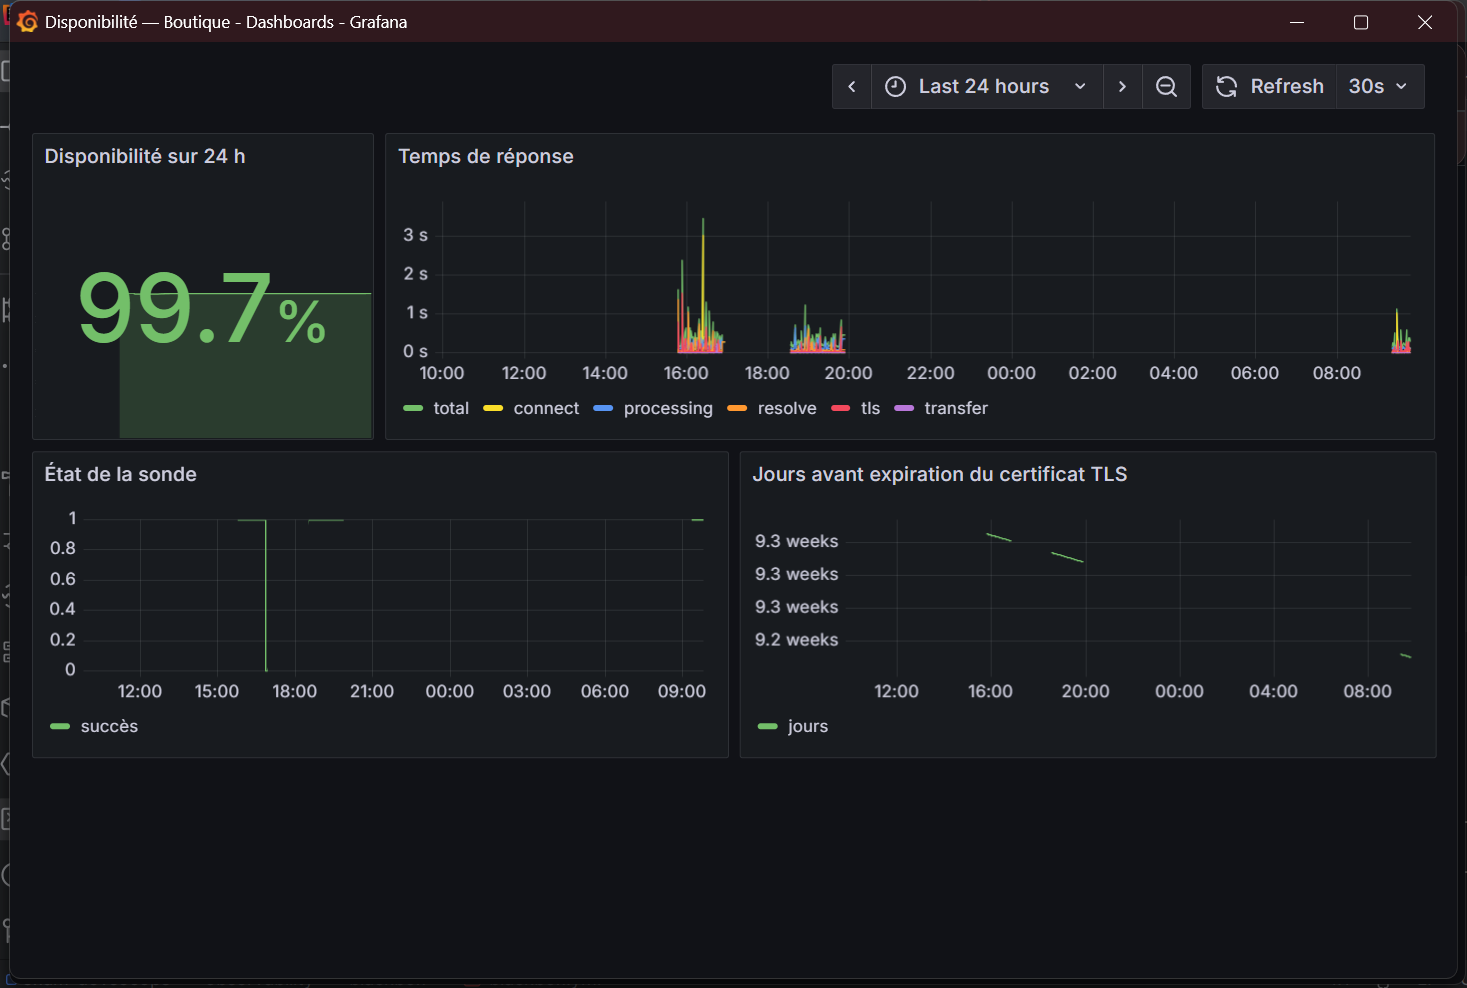
\includegraphics[width=\linewidth]{grafana-disponibilite.png}
\caption{Tableau de bord alimenté par des sondes réelles : disponibilité sur
24~heures, temps de réponse par phase, état de la sonde et jours restants
avant expiration du certificat.}
\end{figure}

\subsection{Une limite mesurée, et non masquée}

L'offre gratuite suspend le service après quinze minutes sans trafic. Les
sondes l'enregistrent : creux de disponibilité et pics de latence à chaque
reprise d'activité.

\textbf{Ce n'est pas un défaut à dissimuler} : c'est le premier constat que
produit une chaîne d'observabilité qui fonctionne. Il est traité comme tout
indicateur dégradé — constat chiffré, cause identifiée par sa signature,
remède connu. Le contournement par maintien en éveil est écarté : il
verdirait le tableau de bord au prix de la validité de la mesure.

% =====================================================================
\section{Conclusion : limites actuelles et améliorations futures}
% =====================================================================

La chaîne remplit ses quatre objectifs : une modification fusionnée arrive
en ligne sans intervention manuelle et avec une mise en ligne vérifiée ;
onze contrôles bloquants la précèdent ; aucun secret ne réside dans le dépôt
ni dans l'image ; et l'ensemble se rejoue depuis le dépôt seul.

Elle a aussi des limites, énoncées ici avec leur remède — une limite connue
et mesurée coûte toujours moins cher qu'une limite ignorée.

\subsection{La limite principale : l'artefact déployé n'est pas l'artefact scanné}

La conception prévoyait que la plateforme tire l'image par son digest,
établissant par empreinte cryptographique que ce qui est en ligne est
exactement ce qui a été validé. Le service disponible sur l'offre gratuite
est adossé au dépôt Git : il reconstruit l'image depuis le
\texttt{Dockerfile} du commit courant et n'accepte pas qu'on lui impose une
image précise.

\textbf{Ce qui subsiste} — le déploiement ne s'exécute que si le scan a
réussi \emph{sur ce même commit}, et l'image scannée est publiée sur GHCR,
donc archivée et vérifiable. \textbf{Ce qui est perdu} — la preuve que
l'artefact servi est le même objet, et non son équivalent reconstruit depuis
la même source.

C'est la seule limite du projet qui touche à une propriété de sécurité
démontrable plutôt qu'à un confort d'exploitation. Toutes les autres
ajoutent de la couverture ; celle-là restaure une preuve. Son remède est
aussi le plus simple : un service de type \textit{image-backed} rétablit la
garantie sans autre modification du pipeline.

\subsection{Les autres limites}

\begin{table}[htbp]
\centering
\small
\begin{tabular}{@{}l l l@{}}
\toprule
\textbf{Limite} & \textbf{Conséquence} & \textbf{Remède} \\
\midrule
Suspension après 15 min    & Latence de réveil mesurée   & Offre payante \\
Jeton côté client          & Lisible par script injecté  & Cookie \texttt{HttpOnly} via BFF \\
Image non signée           & Substitution indétectable   & Cosign \\
Pas de SBOM                & Réponse lente à une CVE     & Syft \\
Pas de test E2E            & Parcours cassé non vu       & Playwright, 3 parcours \\
Pas de retour arrière      & Rollback manuel             & Tâche sur échec de sonde \\
API tierce sans garantie   & Catalogue vide si panne     & État d'erreur explicite \\
Panier non persistant      & Perdu au rafraîchissement   & Sérialiser le réducteur \\
Alertes sans destinataire  & Personne n'est prévenu      & Alertmanager \\
\bottomrule
\end{tabular}
\caption{Limites connues et remède identifié pour chacune}
\label{tab:limites}
\end{table}

Trois de ces remèdes ne coûtent que deux étapes de workflow et aucun secret
supplémentaire : Cosign, Syft et le retour arrière automatique. Deux
supposent un arbitrage financier — l'offre payante lève à la fois la
suspension et la limite principale ci-dessus. Le dernier, Alertmanager, est
reporté pour une raison de principe : il exige un secret de destination,
donc une configuration que personne ne pourrait rejouer à l'identique depuis
le dépôt seul.

\subsection*{Ce que la chaîne enseigne}

Une chaîne d'observabilité qui fonctionne commence par afficher des
indicateurs dégradés — et c'est le signe qu'elle mesure quelque chose. Un
tableau de bord toujours vert est presque toujours un tableau de bord qui ne
mesure rien.

\end{document}
